\chapter{The Encounter in Madrid}
\vspace{0.6cm}
\begin{center}
\nopagebreak
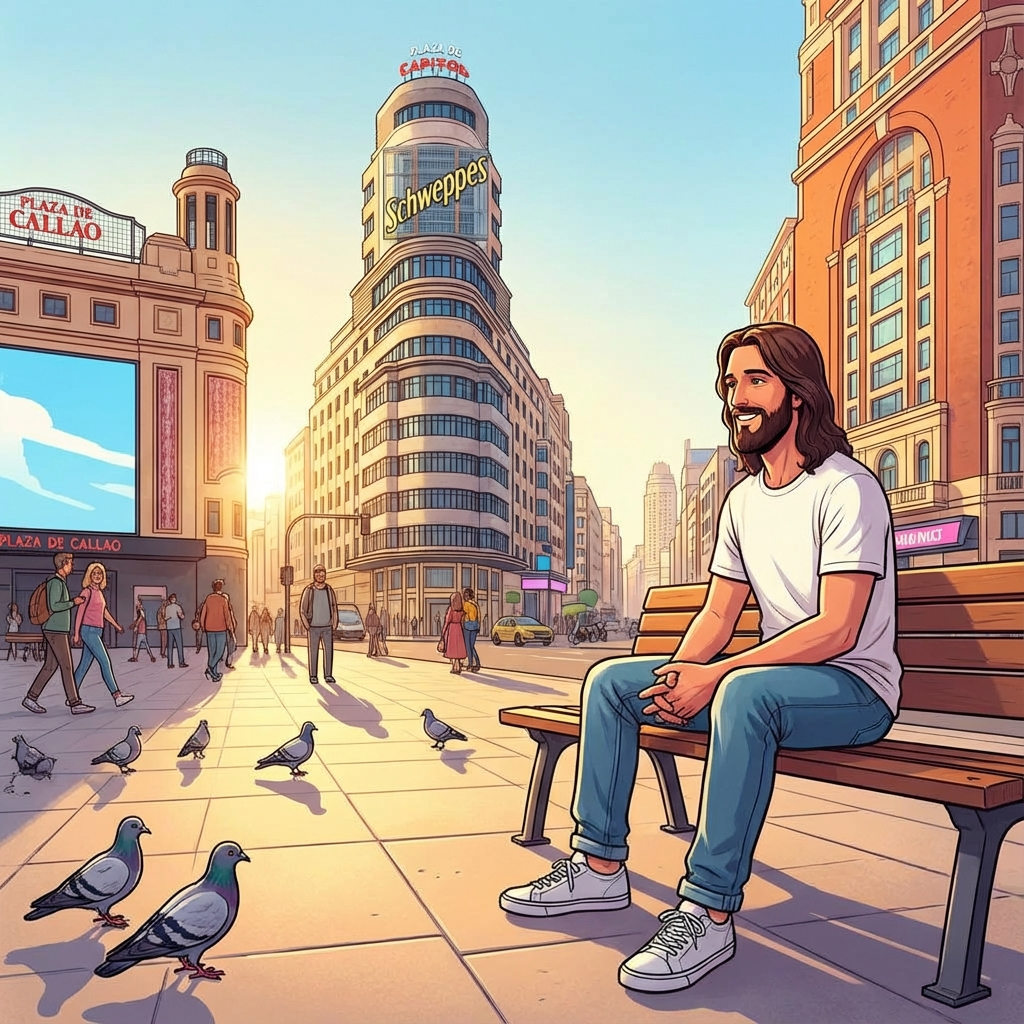
\includegraphics[width=0.75\textwidth,cfbox=gray!60 0.6pt 4pt]{madrid.png}\\
\vspace{4pt}
{\small\itshape Meeting in the city: living presence in everyday life.}
\end{center}

\vspace{0.6cm}
It was a spring afternoon in Madrid. The sun filtered through the buildings of the Gran Vía, creating games of light and shadow that seemed to dance on the asphalt. I was walking with the usual haste of someone living in the city, with a mind full of noise: emails to answer, bills, worries... vibrating low, very low.


Suddenly, in Callao square, I saw him. He wasn't wearing a tunic, nor sandals, nor did he have a shining halo over his head. He was wearing worn-out jeans, a white t-shirt, and comfortable sneakers. He was sitting on a bench, watching people pass by with a calm smile, a smile that seemed to stop time.


—Hello, Francisco —he said when I passed close by.


I stopped dead in my tracks. No one called me by my full name in the street, and certainly not a stranger. But looking into his eyes, I knew he wasn't a stranger. There was an ancestral familiarity in his gaze, a peace that disarmed any defense.


—Jesus? —I asked, feeling a bit ridiculous.


—The same —he replied, patting the empty space on the bench beside him—. Sit down for a while. You are vibrating at a frequency that is giving me a headache, and I can endure a lot.


I sat down, still stunned.
—Vibrating? —I repeated.


—Yes, vibrating. Everything is vibration, my friend. Fear, haste, anger... are dense, heavy vibrations. They anchor you to the ground and don't let you see the sky, even if you have it right above you.


I looked up. The sky in Madrid was an intense, beautiful blue. I hadn't noticed it until that moment.


—I've come to spend a few days with you —he continued—. Let's go for a walk. You need to remember how to tune the radio of your soul. You are listening to pure static.


And so, in the middle of the bustle of Madrid, began the strangest and most wonderful adventure of my life. Not with miracles of turning water into wine, but with the miracle of transforming my internal noise into music.